\chapter{Analysis framework}

To construct a framework for general Particle Flow analysis and data Monte Carlo comparison a large amount of ingredients is needed to be included and checked to be correctly working. In this chapter I will go over the important tools included in my framework. The impact of every given tool will be demonstrated and possible problems in current implementation are also included to summarize the status of the framework.

%should the event selection be here ?

\section{Jet cleaning}

The Jet cleaning allows to apply certain requirements on jets in an event and therefore to remove jets or even complete events that might be bad data. The Jet Cleaning is used on both data and Monte Carlo to make sure that Monte Carlo events that would be removed in data also are not included in the simulation.

\section{The Good Run List}

The Good Run List is only needed for actual detector data. For data to be suitable fo analysis one has to make sure that it fits certain requirements of which some depend on the detectors working state. The Good Run List allows to exclude data-taking periods in which the detector showed a poor working state. Reasons for this may be maintenance on sub detectors, magnets off or ramping or an unstable beam of the LHC.
The Good Run List includes all the good data taking periods and the tool excludes all data from bad periods.

\section{Jet Calibration and Smearing}

After making sure a Jet is "good" and therefore has passed the cleaning it must still be be calibrated and in case of MC smeared to data. The Calibration scales the energy of jets for a certain reconstruction algorithm. The Smearing smears the MC resolution to be matching the actual data resolution.


\begin{figure}
\centering
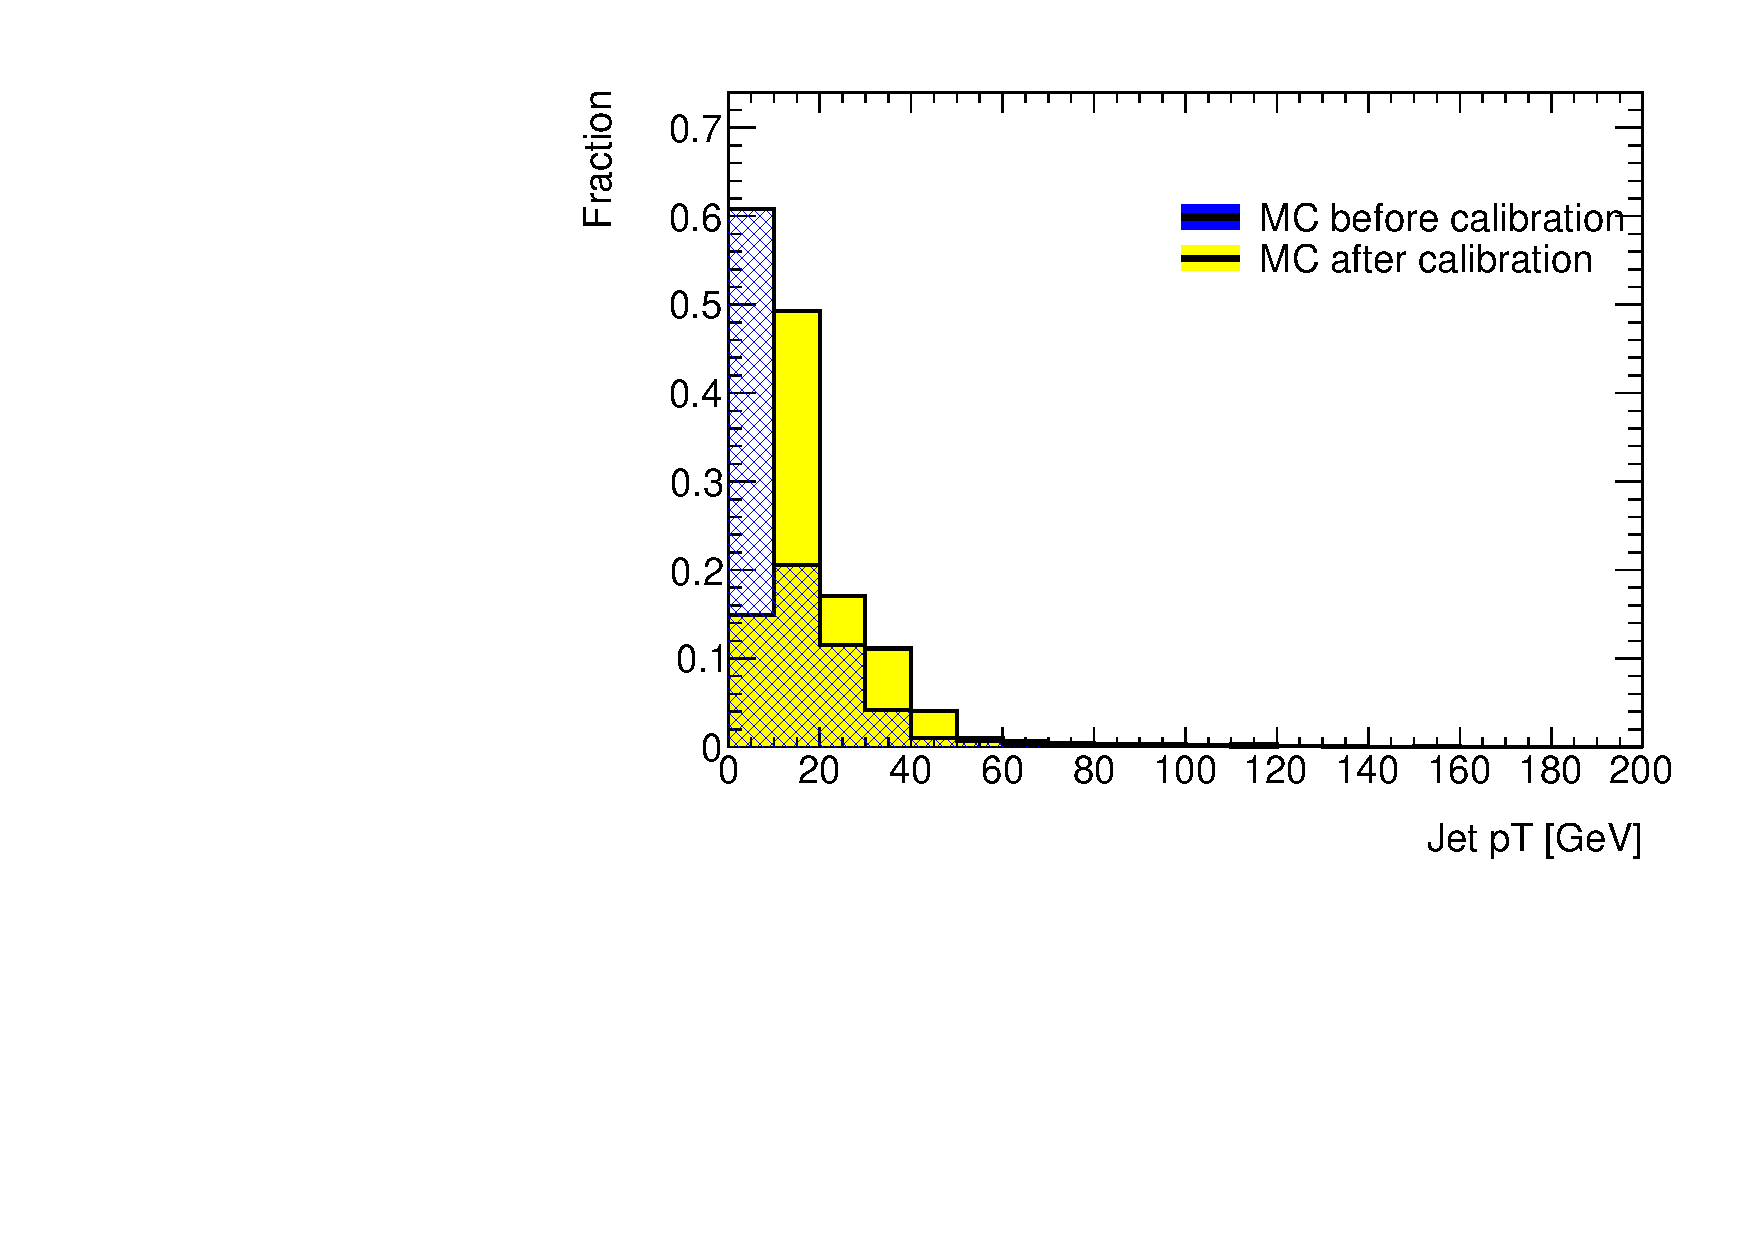
\includegraphics[width=\figwidth]{testscalingpt}
\caption[Influence of the JES on the transversal momentum]{The influence of the calibration in momentum is shown}
\label{fig:testscalingpt}
\end{figure}

\begin{figure}
\centering
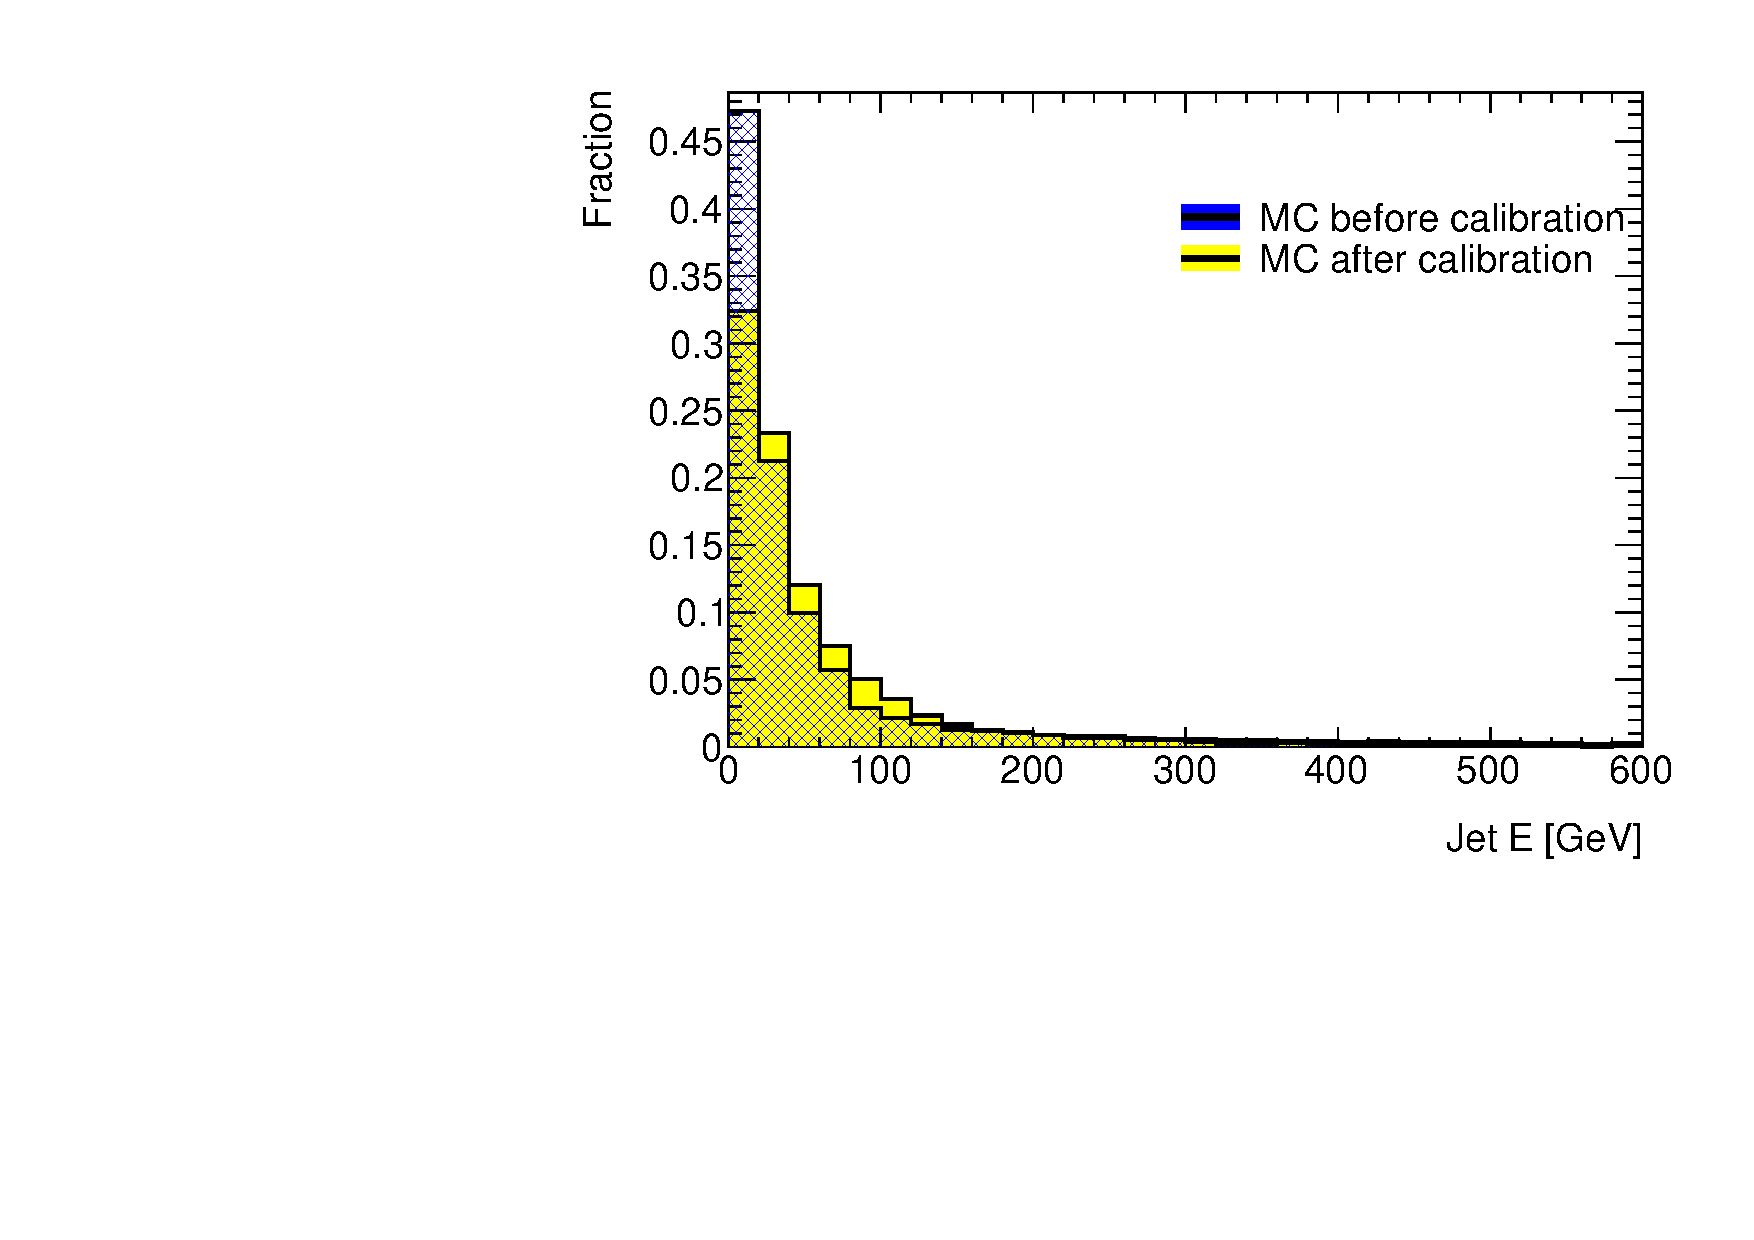
\includegraphics[width=\figwidth]{testscalinge}
\caption[Influence of the JES on the energy]{The influence of the calibration in energy is shown}
\label{fig:testscalinge}
\end{figure}


\begin{figure}
\centering
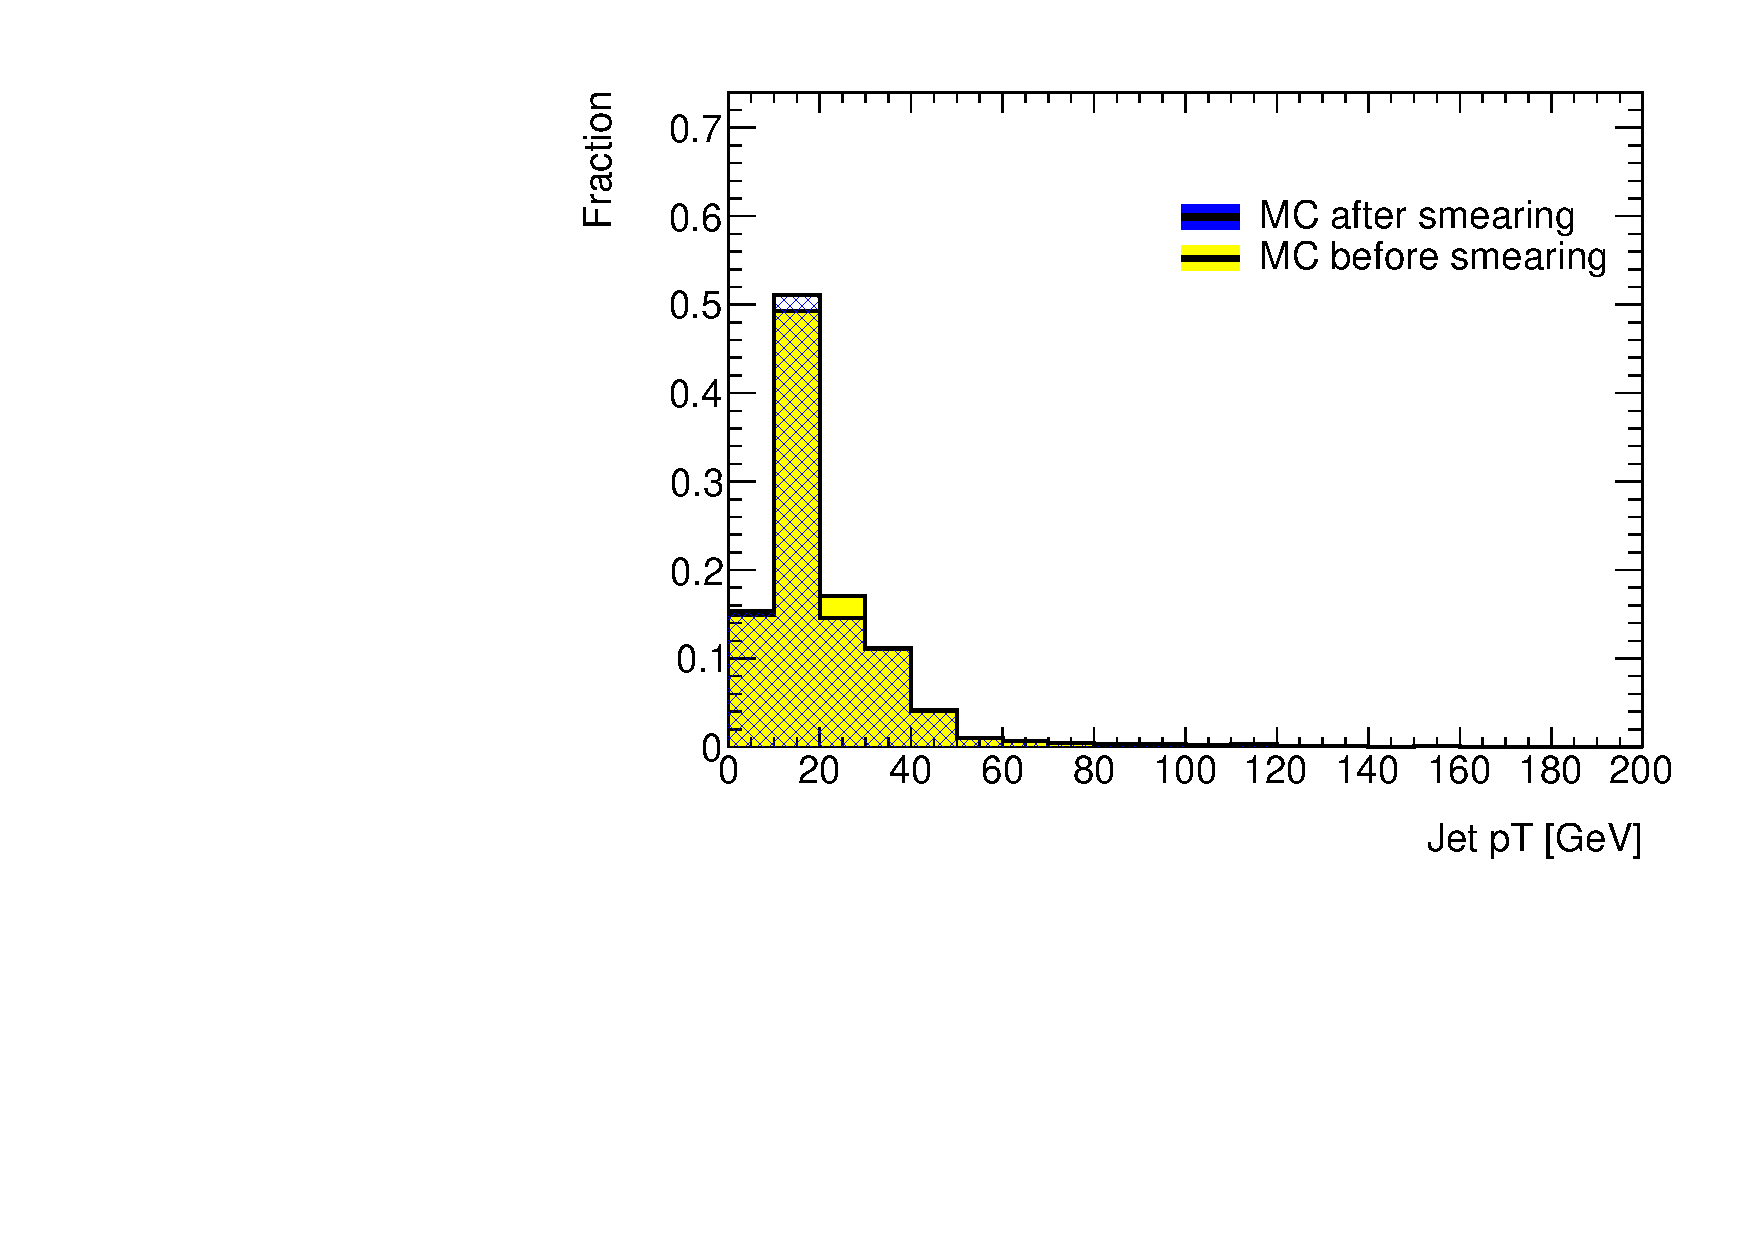
\includegraphics[width=\figwidth]{testsmearingpt}
\caption[Influence of the Smearing on the transversal momentum]{The influence of the Smearing in momentum is shown}
\label{fig:testsmearingpt}
\end{figure}

\begin{figure}
\centering
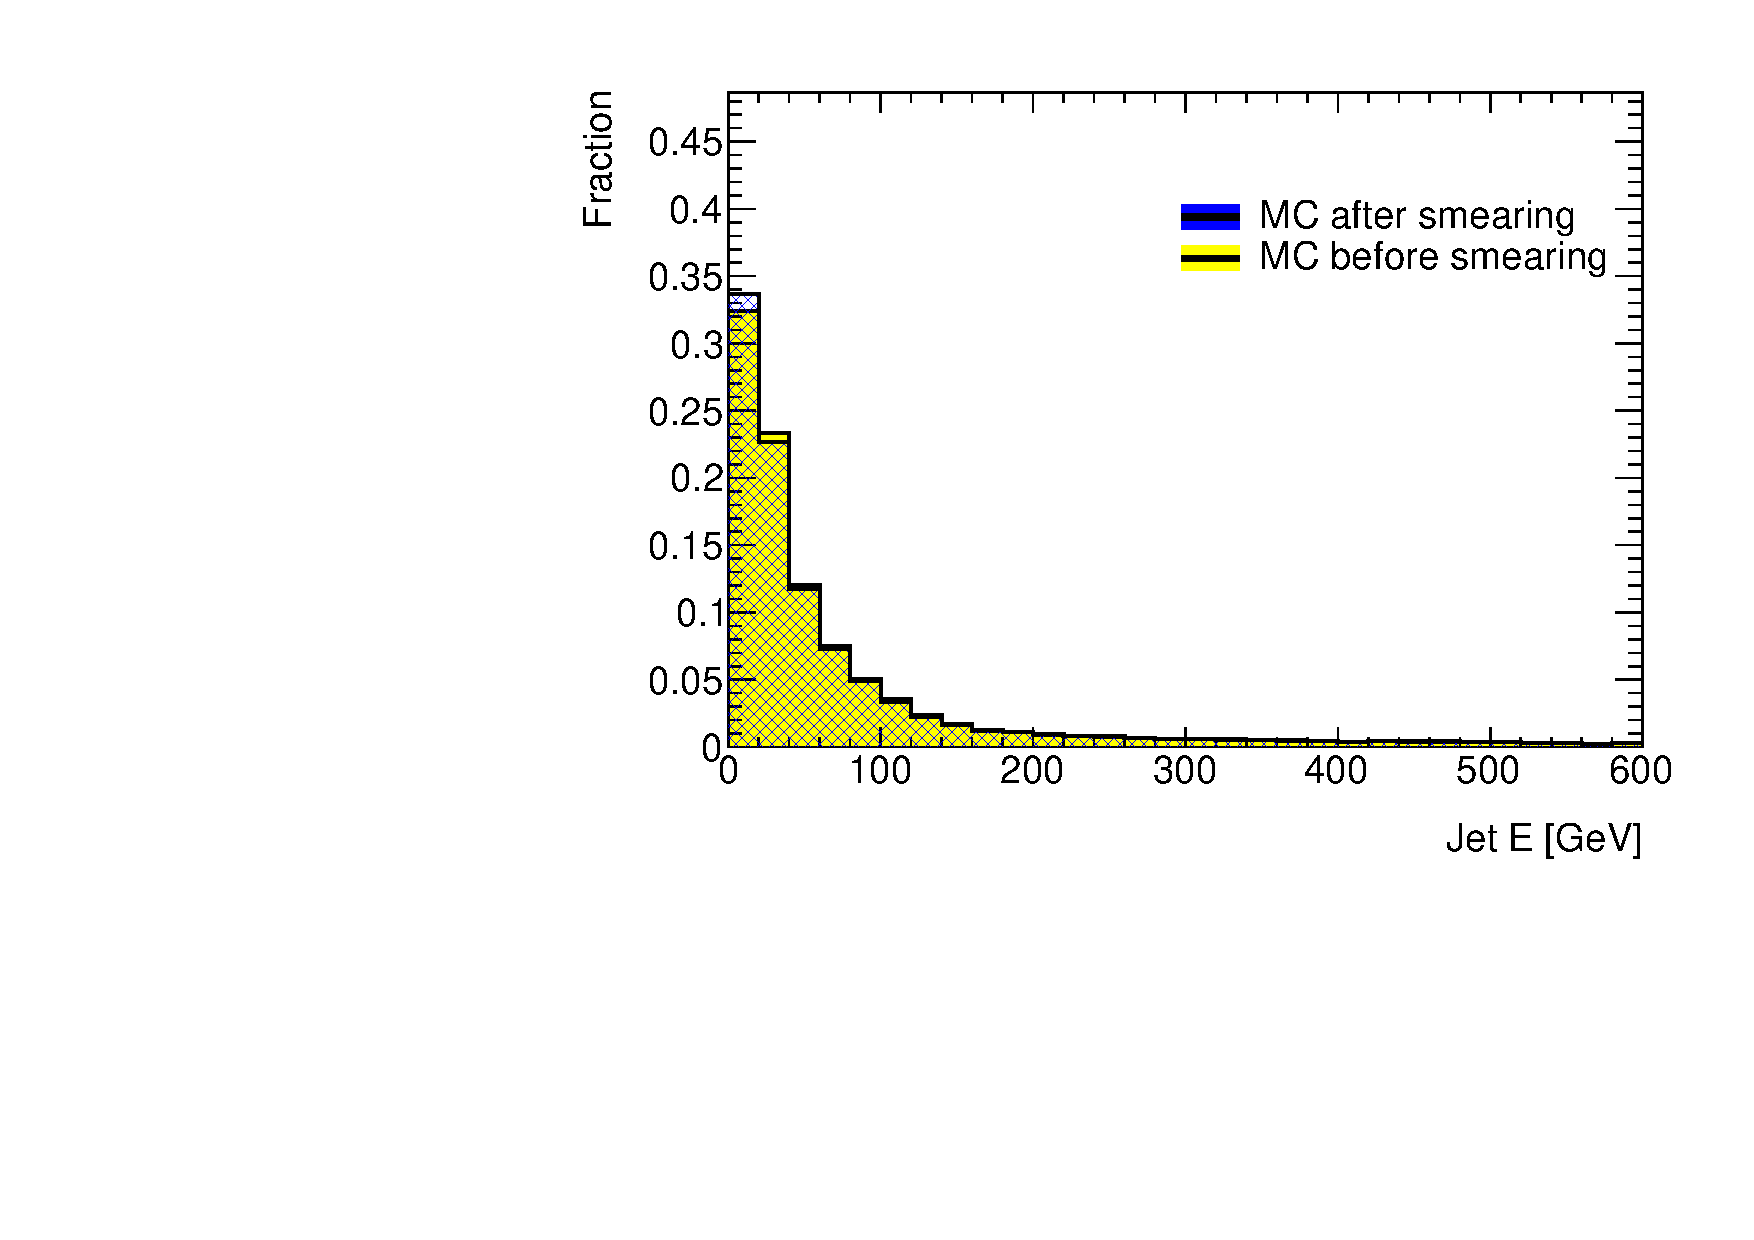
\includegraphics[width=\figwidth]{testsmearinge}
\caption[Influence of the Smearing on the energy]{The influence of the Smearing in energy is shown}
\label{fig:testsmearinge}
\end{figure}



\section{The jet vertex tagger}

An important part of analysis is the rejection of pileup jets. A way to minimize pilup is to calculate the jet-vertex fraction of each jet which is the fraction of momentum in the jet originating from the primary vertex. If one sets a minimum on this fraction pileup can be suppressed. The Jet Vertex Tagger related each jet to a vertex.

\section{Trigger Tools}

A further important collection of tools has to make sure that the trigger is fired, correctly used and also that the particle that triggered is actually one of those used in later analysis.

A trigger basically is a first selection for an event meaning that an event is required to surpass certain demands to be used in analysis. These demands are embodied by so called trigger chains that can be used as input for a trigger tool in analysis which on that base can select or refuse events.

Usually the trigger is checked before the event is further cleaned and calibrated. Therefore it can happen that the particles that passed the trigger later get removed in the analysis. The trigger matching makes sure that the particles that passed the triggers are still left in the final analysis and if not the event can still be removed.

\section{Monte Carlo Re-weighting}

The Monte Carlo is produced before data is taken therefore the shape of Monte Carlo may vary from the shape of the actual taken data for several reasons. For example the pileup in MC may not match the data as well as the resolution. To compensate these differences a sum of weights is applied to Monte Carlo.

\section{Data Re-weighting}

\section{Muon Calibration and Selection}

Analog to jets the muons in an event also have to go through several cuts and have to be calibrated properly. This section introduces all the important tools for muon calibration and gives a brief summary of the effects of the cuts and calibrations.

\section{Electron Calibration and Selection}

The electron tools are the more or the less parallel to the muon tools and I will summarize and explain them in the same way.